\chapter {Experiment} %INCLUDE AVERAGES AND CHANGE DP

All of my experiments are carried out using my chosen method discussed in the 'Methods' section on page \pageref{Chosen Method}. The columns highlighted in red are outliers that I will not be using in my 'Analysis and Interpretation' section. All of my experiments are also carried out using 40 cm$^3$ of solution with 1.0 g of zinc, unless otherwise stated.

\section{Non-Catalysed Experiment Series}

In order to work out the order of sulfuric acid in the Zinc and sulfuric acid reaction I carried out an experiment without the presence catalyst. I varied the concentration of the sulfuric acid (6 series with a range of 2.0 Molar - 6.0 Molar) whilst keeping the mass of zinc the same (1.0 g). To make up my solutions I followed the procedure I outlined in my 'Preparing Chemicals' section on page \pageref{Preparing Chemicals}. My raw data tables can be seen below for each concentration of sulfuric acid.

	\subsection{2.0 Molar Sulfuric Acid}

\begin{figure}[H]
    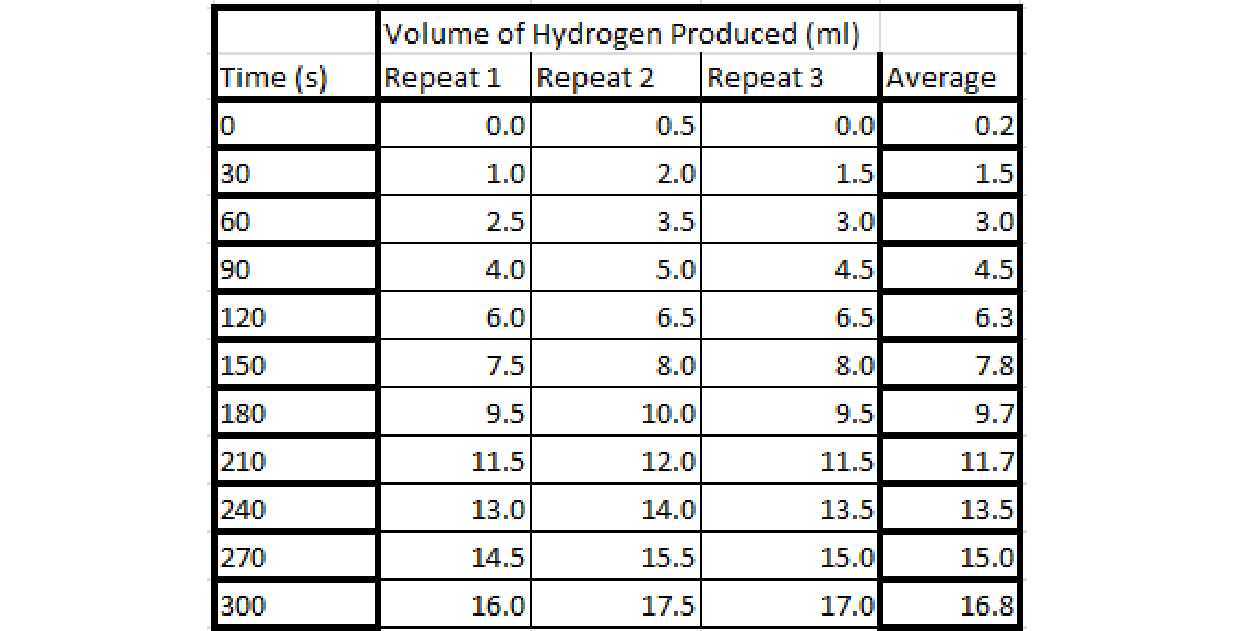
\includegraphics[width=\textwidth]{./Experiment/Images/1NonCatalyst/2Molar.pdf}
    \caption{2 Molar Sulfuric Acid and 1.0 g of Zinc} \label{fig:2MolarSARawData}
\end{figure}


	\subsection{2.4 Molar Sulfuric Acid}

\begin{figure}[H]
    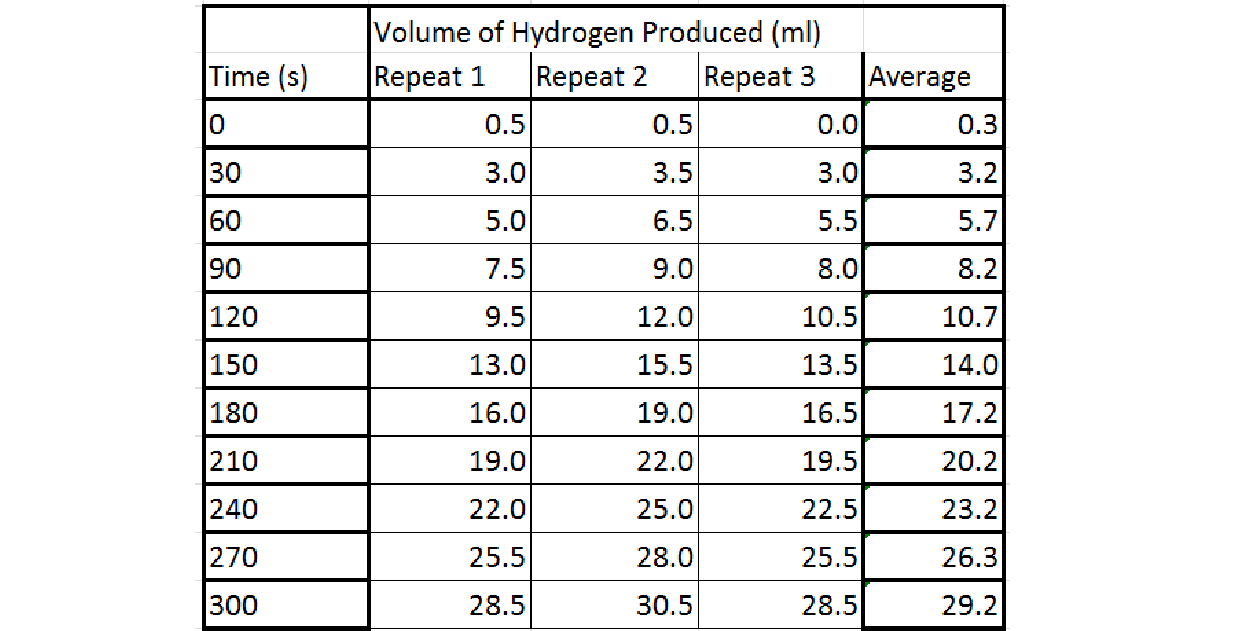
\includegraphics[width=\textwidth]{./Experiment/Images/1NonCatalyst/24Molar.pdf}
    \caption{2.4 Molar Sulfuric Acid and 1.0 g of Zinc} \label{fig:24MolarSARawData}
\end{figure}

	\subsection{2.8 Molar Sulfuric Acid}

\begin{figure}[H]
    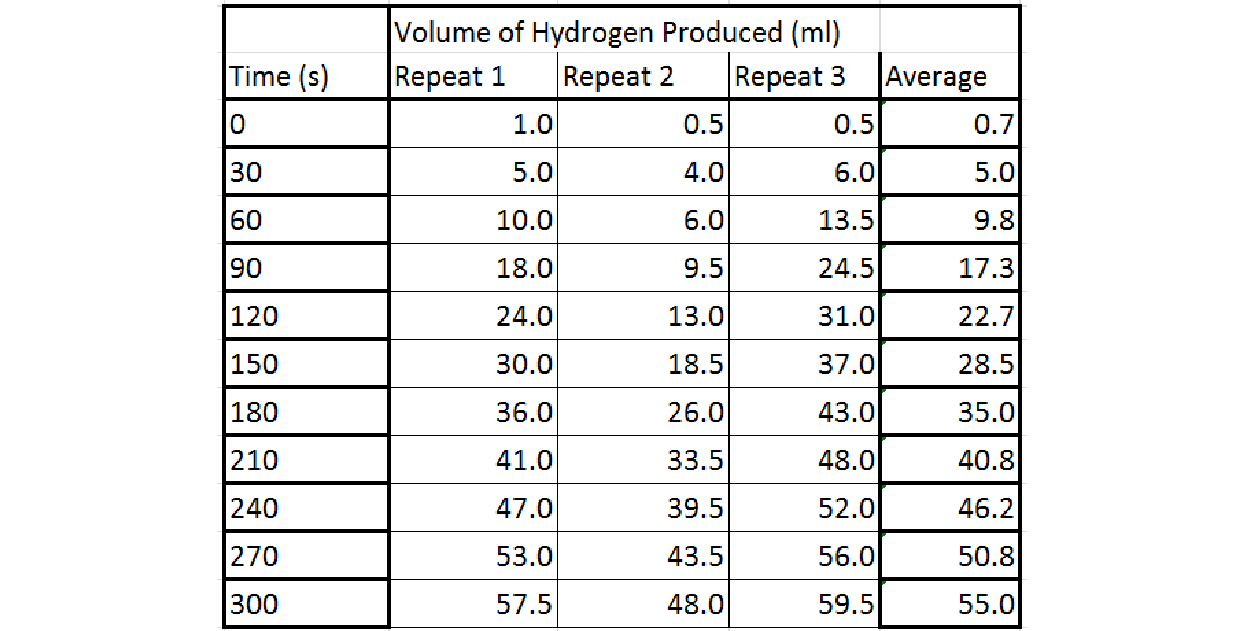
\includegraphics[width=\textwidth]{./Experiment/Images/1NonCatalyst/28Molar.pdf}
    \caption{2.8 Molar Sulfuric Acid and 1.0 g of Zinc} \label{fig:28MolarSARawData}
\end{figure}

	\subsection{3.2 Molar Sulfuric Acid}

\begin{figure}[H]
    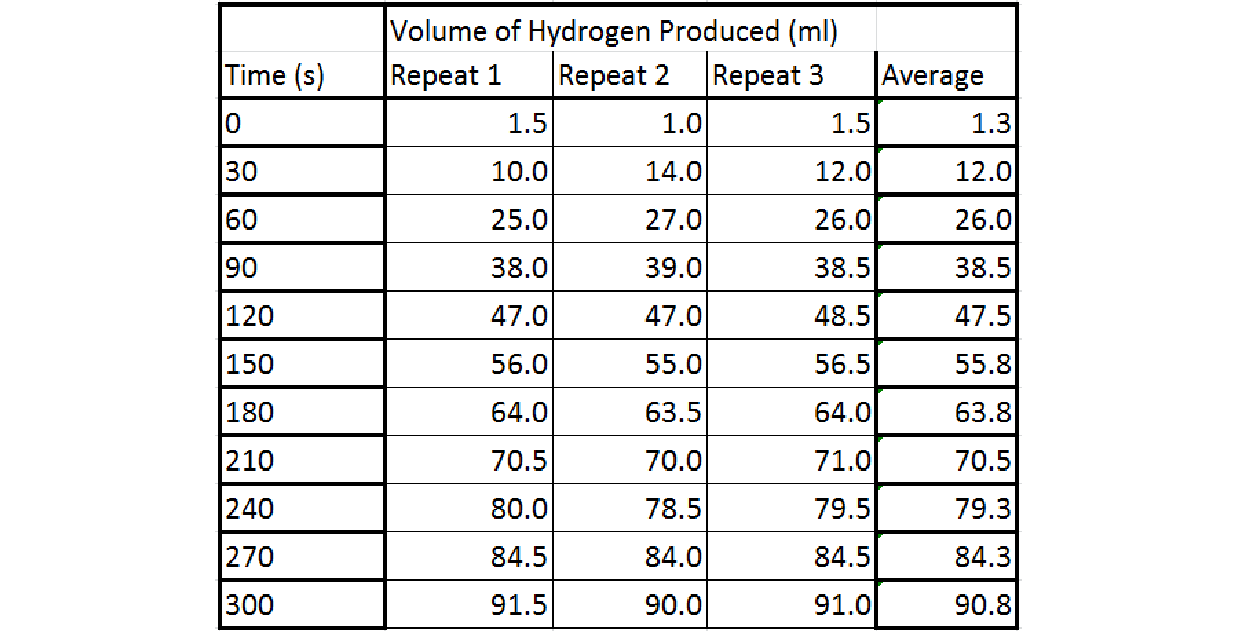
\includegraphics[width=\textwidth]{./Experiment/Images/1NonCatalyst/32Molar.pdf}
    \caption{3.2 Molar Sulfuric Acid and 1.0 g of Zinc} \label{fig:32MolarSARawData}
\end{figure}

	\subsection{3.6 Molar Sulfuric Acid}

\begin{figure}[H]
    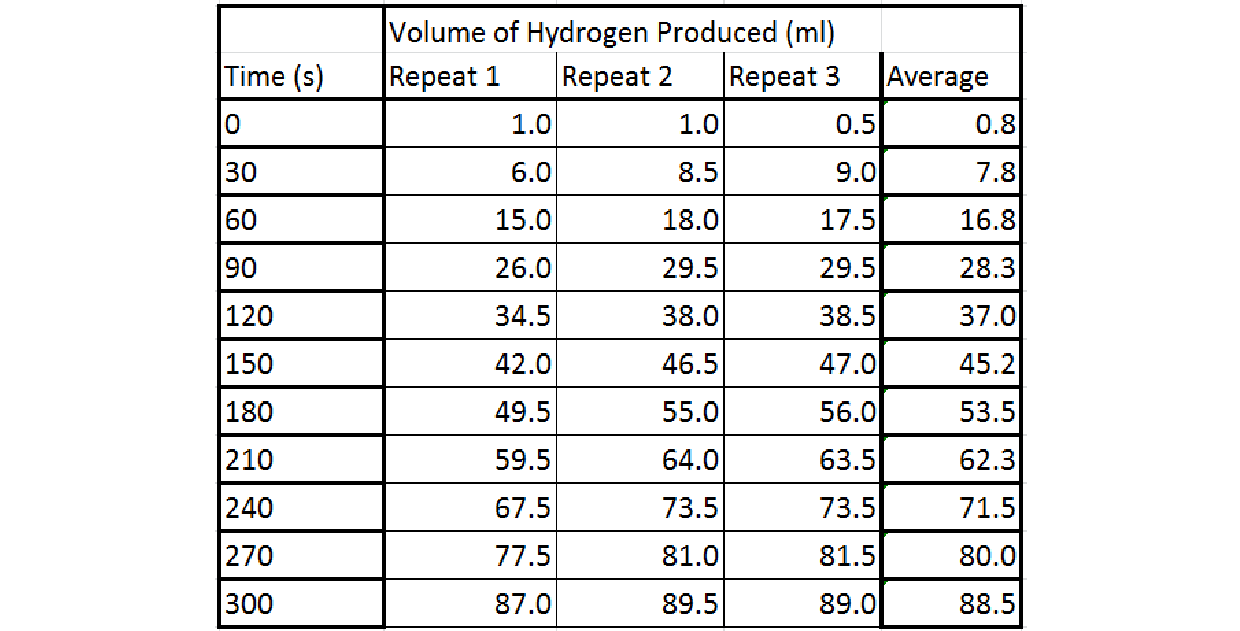
\includegraphics[width=\textwidth]{./Experiment/Images/1NonCatalyst/36Molar.pdf}
    \caption{3.6 Molar Sulfuric Acid and 1.0 g of Zinc} \label{fig:36MolarSARawData}
\end{figure}

	\subsection{4.0 Molar Sulfuric Acid}

\begin{figure}[H]
    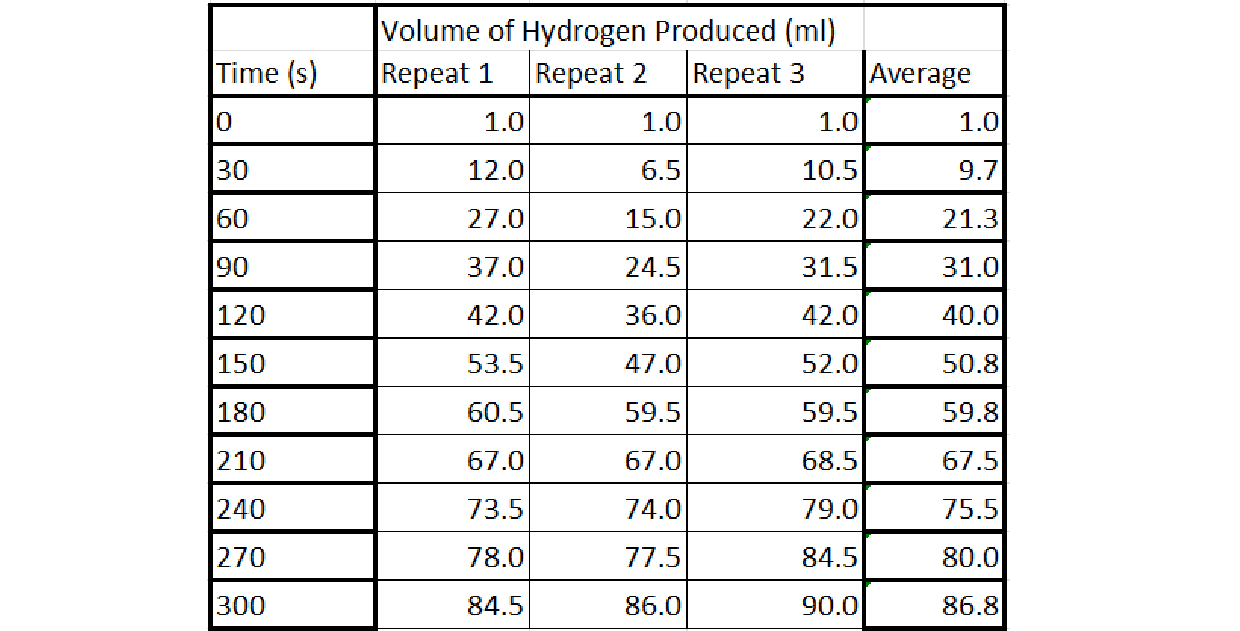
\includegraphics[width=\textwidth]{./Experiment/Images/1NonCatalyst/40Molar.pdf}
    \caption{4.0 Molar Sulfuric Acid and 1.0 g of Zinc} \label{fig:40MolarSARawData}
\end{figure}

\section{Copper Sulfate Catalysed Experiment Series}

My previous experiment series was carried out so that I would be able to work out the order of sulfuric acid without the presence of a catalyst; however the acid may be a different order in presence of a catalyst. For this experiment series I have created 40 cm$^3$, 0.01 molar copper sulfate and a varying concentration of sulfuric acid (6 series from 0.2 molar - 1.2 molar). I prepared these solutions by adding the desired amount of sulfuric acid to make the solution and then adding 10 cm$^3$ of 0.1 molar copper sulfate (which I prepared, as outlined in the 'Preparing Chemicals' section on page \pageref{Preparing Chemicals}), both using a volumetric pipette to carry out the measurements. After the two chemicals were in the volumetric flask I filled the volumetric flask with distilled water up until the meniscus of the solution was on the line. My raw data tables are shown below for this experiment.

	\subsection{0.2 Molar Sulfuric Acid}

\begin{figure}[H]
    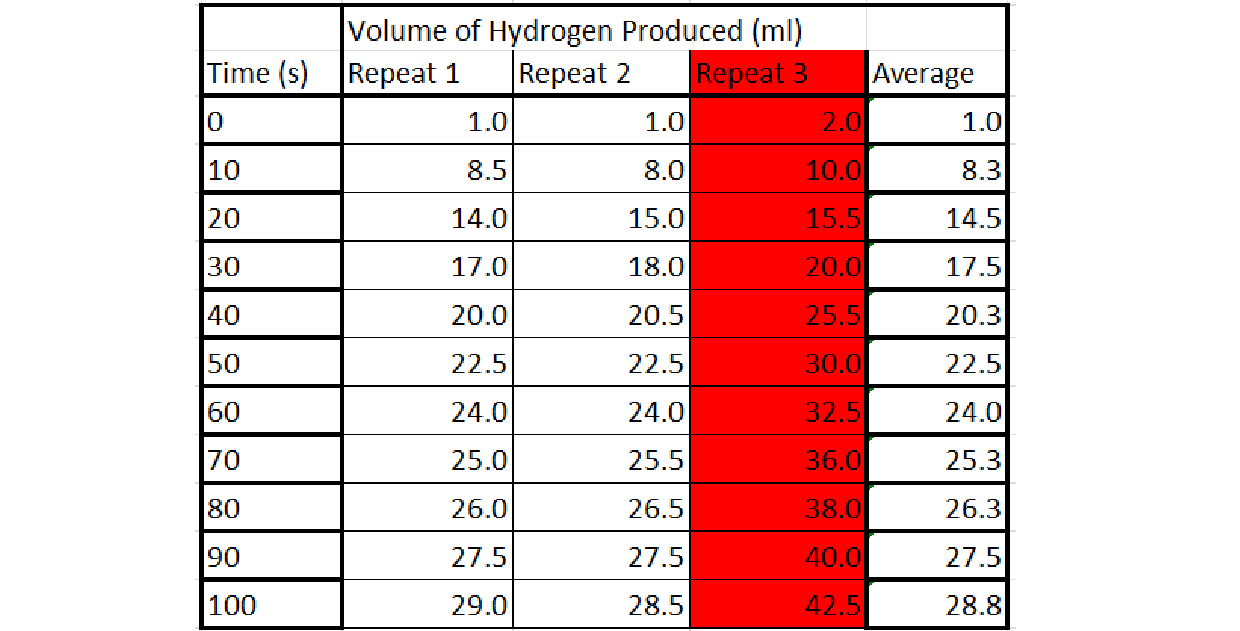
\includegraphics[width=\textwidth]{./Experiment/Images/2FixedCatalyst/02Molar.pdf}
    \caption{0.2 Molar Sulfuric Acid, 0.01 Molar Copper Sulfate and 1.0 g of Zinc} \label{fig:02SACSRawData}
\end{figure}

	\subsection{0.4 Molar Sulfuric Acid}

\begin{figure}[H]
    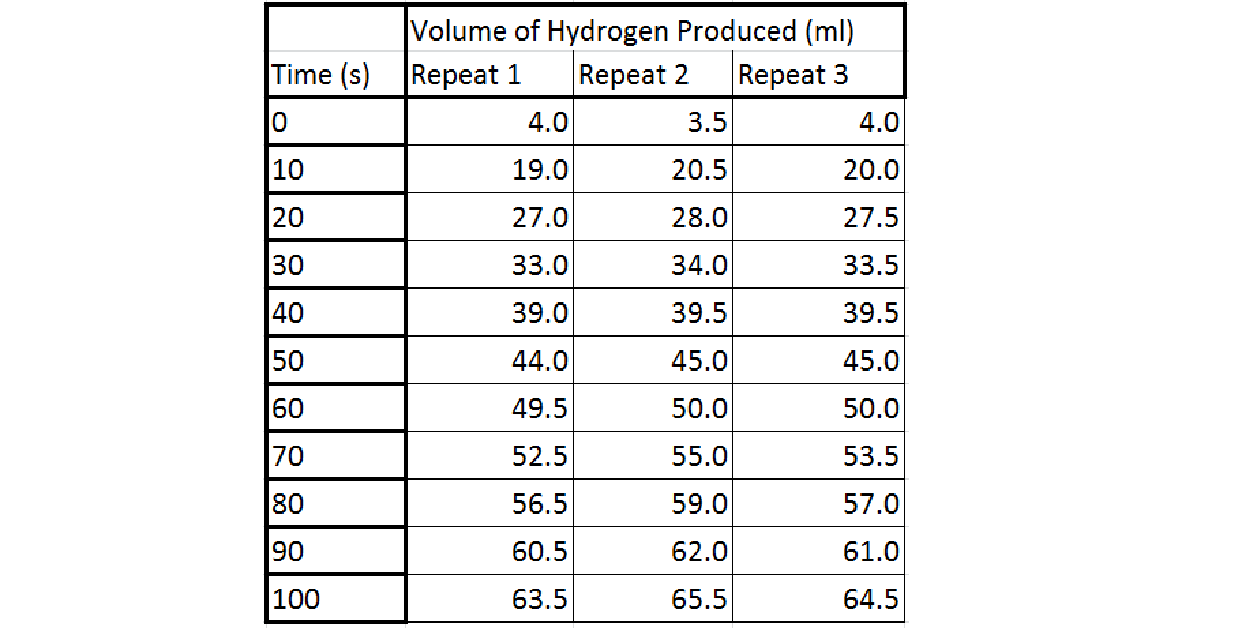
\includegraphics[width=\textwidth]{./Experiment/Images/2FixedCatalyst/04Molar.pdf}
    \caption{0.4 Molar Sulfuric Acid, 0.01 Molar Copper Sulfate and 1.0 g of Zinc} \label{fig:04SACSRawData}
\end{figure}

	\subsection{0.6 Molar Sulfuric Acid}

\begin{figure}[H]
    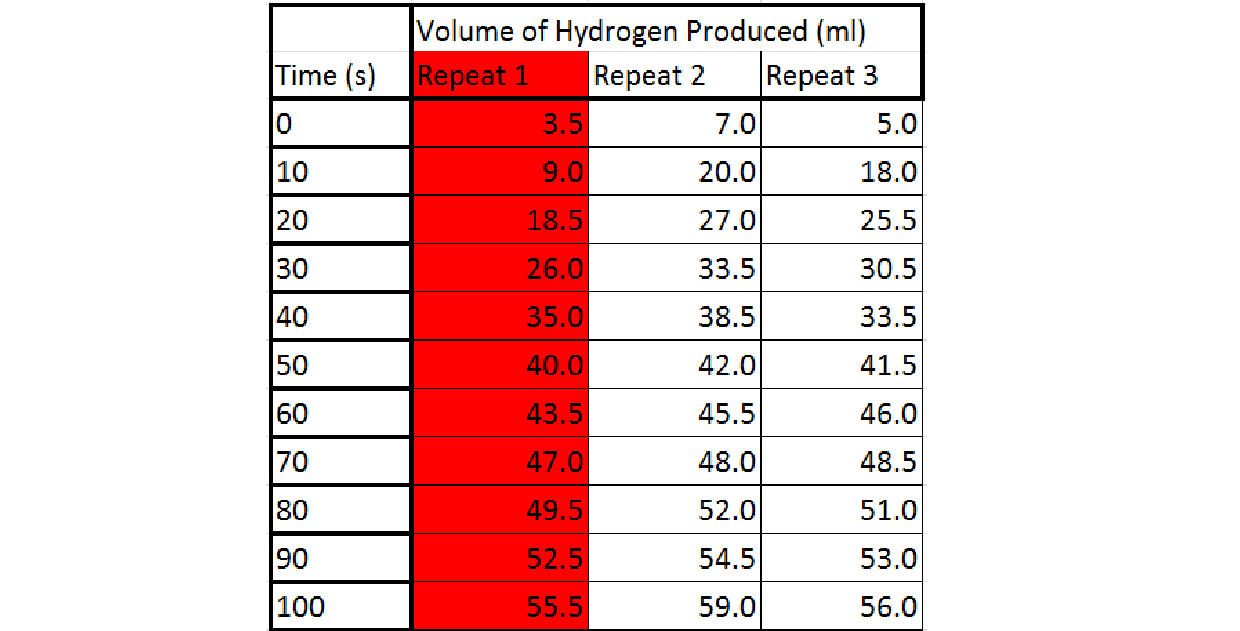
\includegraphics[width=\textwidth]{./Experiment/Images/2FixedCatalyst/06Molar.pdf}
    \caption{0.6 Molar Sulfuric Acid, 0.01 Molar Copper Sulfate and 1.0 g of Zinc} \label{fig:06SACSRawData}
\end{figure}

	\subsection{0.8 Molar Sulfuric Acid}

\begin{figure}[H]
    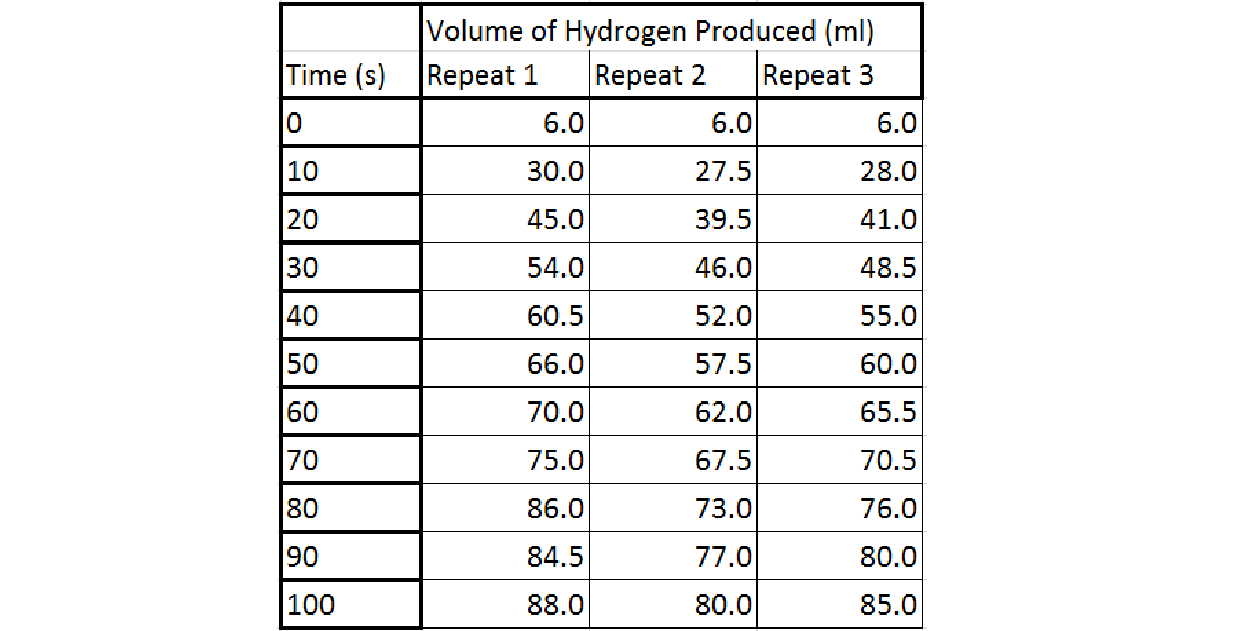
\includegraphics[width=\textwidth]{./Experiment/Images/2FixedCatalyst/08Molar.pdf}
    \caption{0.8 Molar Sulfuric Acid, 0.01 Molar copper sulfate and 1.0 g of Zinc} \label{fig:08SACSRawData}
\end{figure}

	\subsection{1.0 Molar Sulfuric Acid}

\begin{figure}[H]
    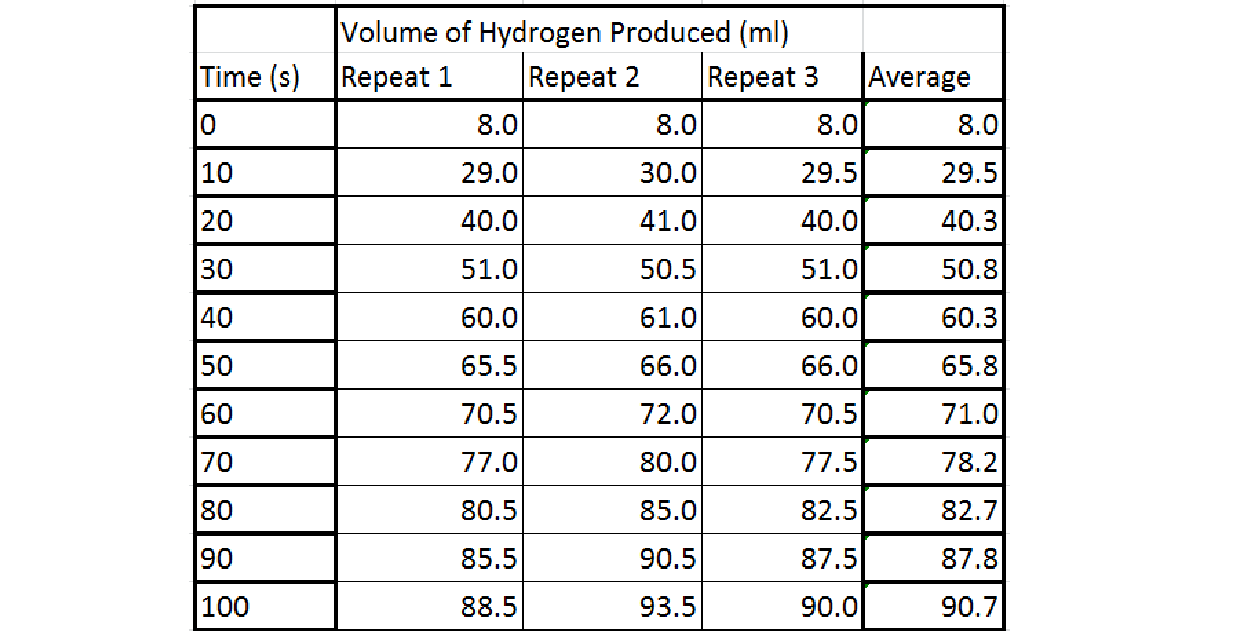
\includegraphics[width=\textwidth]{./Experiment/Images/2FixedCatalyst/10Molar.pdf}
    \caption{1.0 Molar Sulfuric Acid, 0.01 Molar Copper Sulfate and 1.0 g of Zinc} \label{fig:10SACSRawData}
\end{figure}

	\subsection{1.2 Molar Sulfuric Acid}

\begin{figure}[H]
    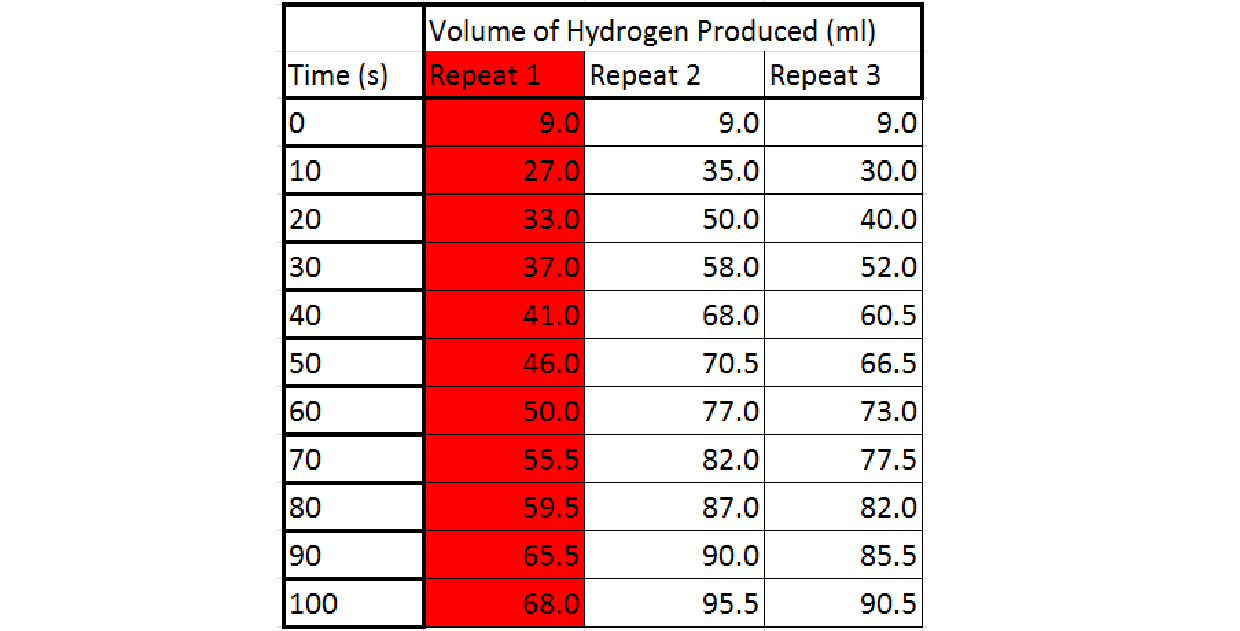
\includegraphics[width=\textwidth]{./Experiment/Images/2FixedCatalyst/12Molar.pdf}
    \caption{1.2 Molar Sulfuric Acid, 0.01 Molar Copper Sulfate and 1.0 g of Zinc} \label{fig:12SACSRawData}
\end{figure}


\section{Varying Copper Sulfate Experiment Series}

As I need to find the order of copper sulfate in the reaction, the next logical experiment was to change the concentration of copper sulfate whilst keeping the sulfuric acid concentration the same. For this experiment I used 0.2 molar sulfuric acid with a range of copper sulfate concentrations (6 series from 0.01 molar - 0.06 molar). I made these solutions up the same way as before, but instead of varying the volume of sulfuric acid I initially added to the volumetric flask, I varied the volume of copper sulfate solution I added.  My raw data tables are shown below for this experiment. 

	\subsection{0.01 Molar Copper Sulfate}

Please see Figure \ref{fig:02SACSRawData} on page \pageref{fig:02SACSRawData} for the raw data table of this experiment series.



	\subsection{0.02 Molar Copper Sulfate}

\begin{figure}[H]
    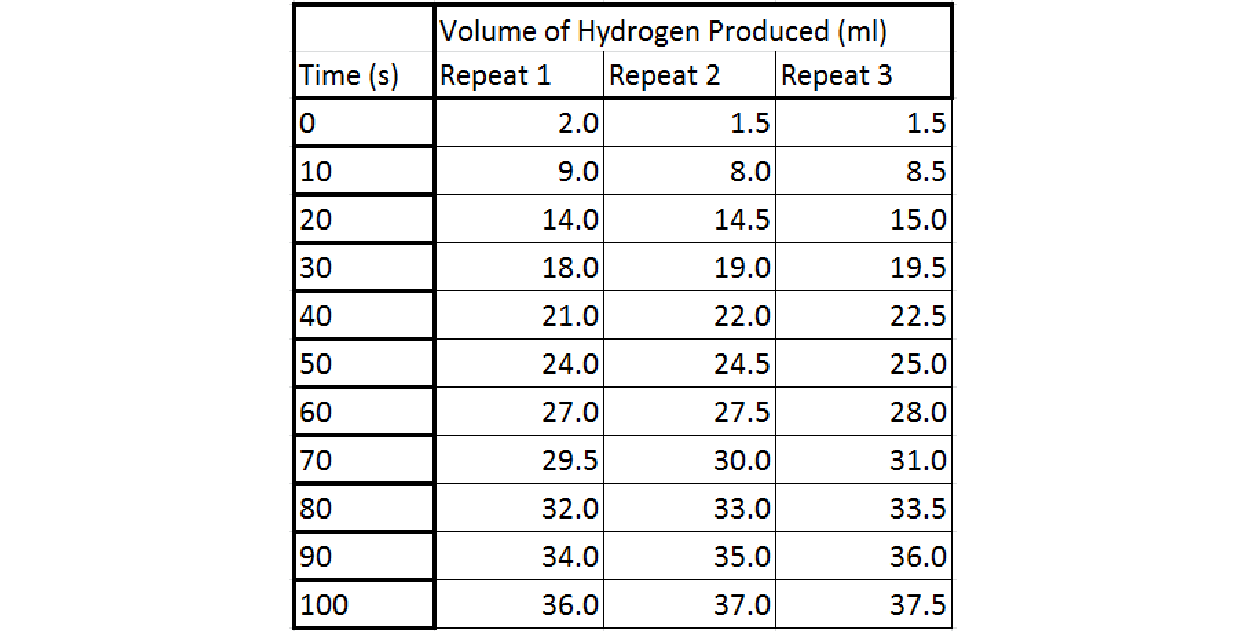
\includegraphics[width=\textwidth]{./Experiment/Images/3ChangeCatalyst/002Molar.pdf}
    \caption{0.2 Molar Sulfuric Acid, 0.02 Molar Copper Sulfate and 1.0 g of Zinc} \label{fig:002MolarCSRawData}
\end{figure}

	\subsection{0.03 Molar Copper Sulfate}

\begin{figure}[H]
    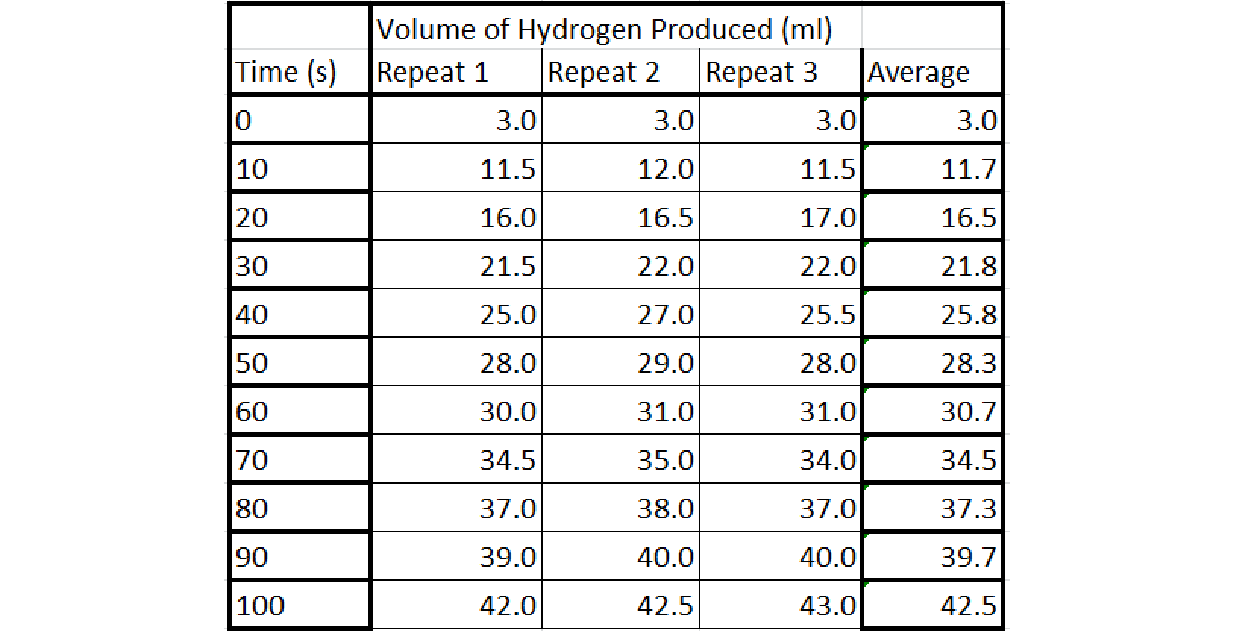
\includegraphics[width=\textwidth]{./Experiment/Images/3ChangeCatalyst/003Molar.pdf}
    \caption{0.2 Molar Sulfuric Acid, 0.03 Molar Copper Sulfate and 1.0 g of Zinc} \label{fig:003MolarCSRawData}
\end{figure}

	\subsection{0.04 Molar Copper Sulfate}

\begin{figure}[H]
    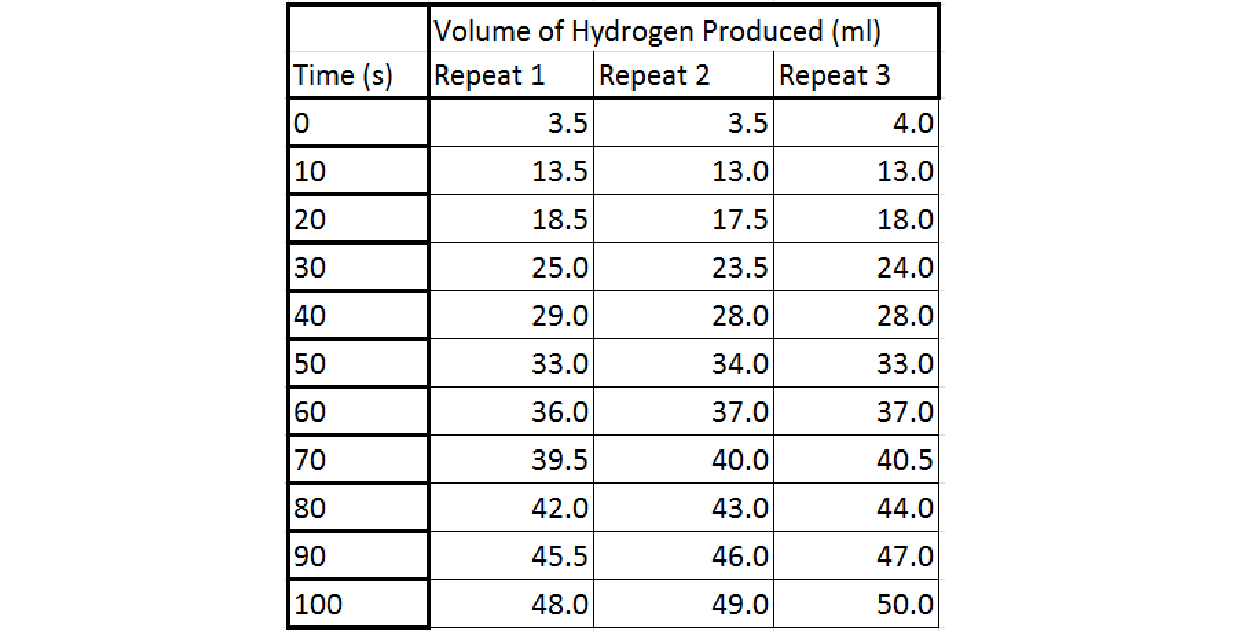
\includegraphics[width=\textwidth]{./Experiment/Images/3ChangeCatalyst/004Molar.pdf}
    \caption{0.2 Molar Sulfuric Acid, 0.04 Molar Copper Sulfate and 1.0 g of Zinc} \label{fig:004MolarCSRawData}
\end{figure}

	\subsection{0.05 Molar Copper Sulfate}

\begin{figure}[H]
    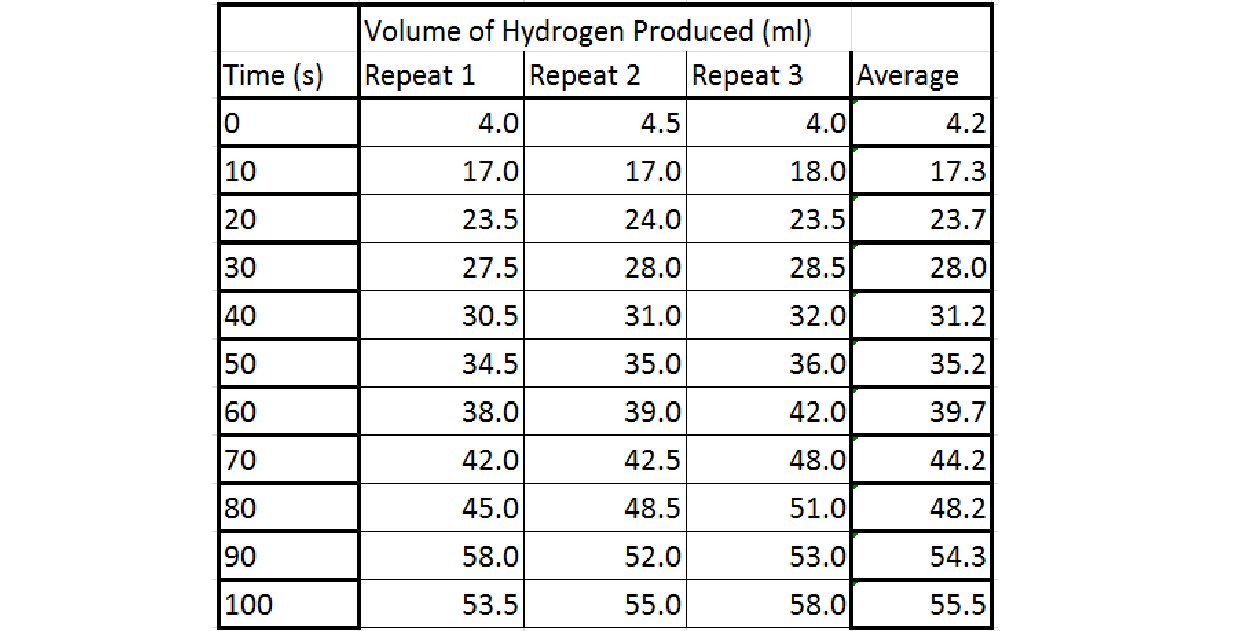
\includegraphics[width=\textwidth]{./Experiment/Images/3ChangeCatalyst/005Molar.pdf}
    \caption{0.2 Molar Sulfuric Acid, 0.05 Molar Copper Sulfate and 1.0 g of Zinc} \label{fig:005MolarCSRawData}
\end{figure}

	\subsection{0.06 Molar Copper Sulfate}

\begin{figure}[H]
    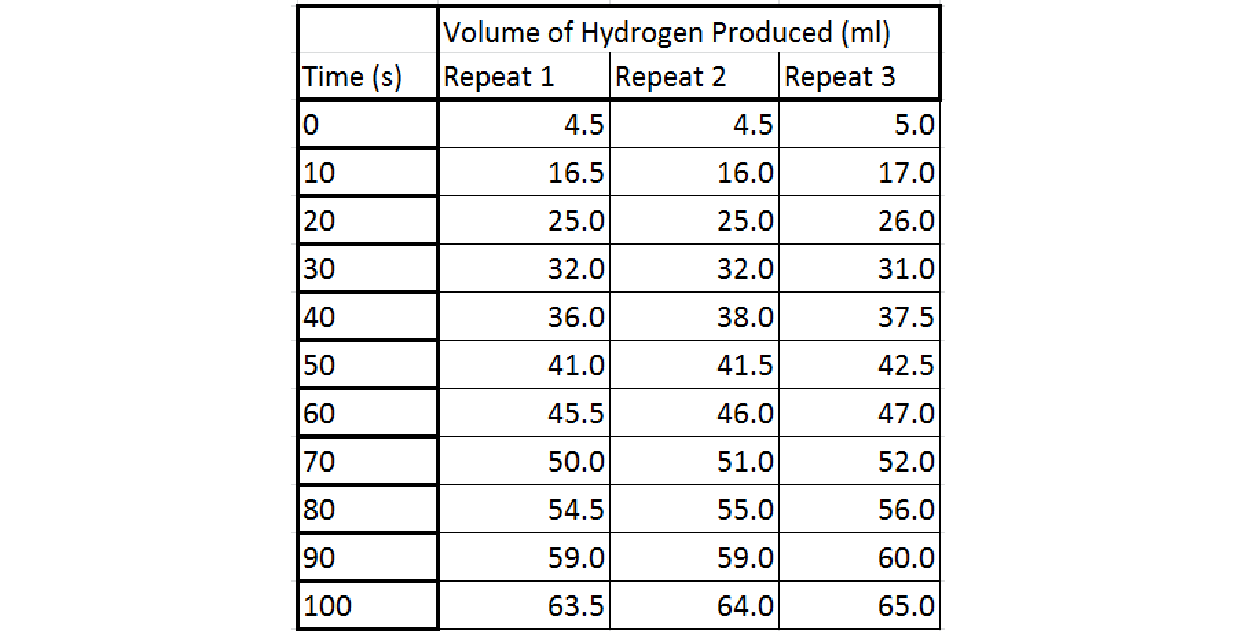
\includegraphics[width=\textwidth]{./Experiment/Images/3ChangeCatalyst/006Molar.pdf}
    \caption{0.2 Molar Sulfuric Acid, 0.06 Molar Copper Sulfate and 1.0 g of Zinc} \label{fig:006MolarCSRawData}
\end{figure}



\section{Different Catalysts Experiment Series}

After finishing my initial experiment, I began to think about how different catalysts affect the rate of reaction. As my college had a low stock of chemicals by the time I began this experiment, I could only get 4 different metal sulfates. These are listed below.

\begin{itemize}
\item Copper Sulfate
\item Nickel Sulfate
\item Manganese Sulfate
\item Iron Sulfate
\end{itemize}

I made up the solutions using 0.4 molar sulfuric acid and 0.01 molar of the catalyst. These were made up using the same method as I used for the rest of my solutions. This can be found in the 'Preparing Chemicals' section on page \pageref{Preparing Chemicals}.

	\subsection{Copper Sulfate}

As the rest of my experiments in this series only have one repeat, I have decided to take the average of the 3 repeats from Figure \ref{fig:04SACSRawData} on page \pageref{fig:04SACSRawData} for the table shown below.

\begin{figure}[H]
    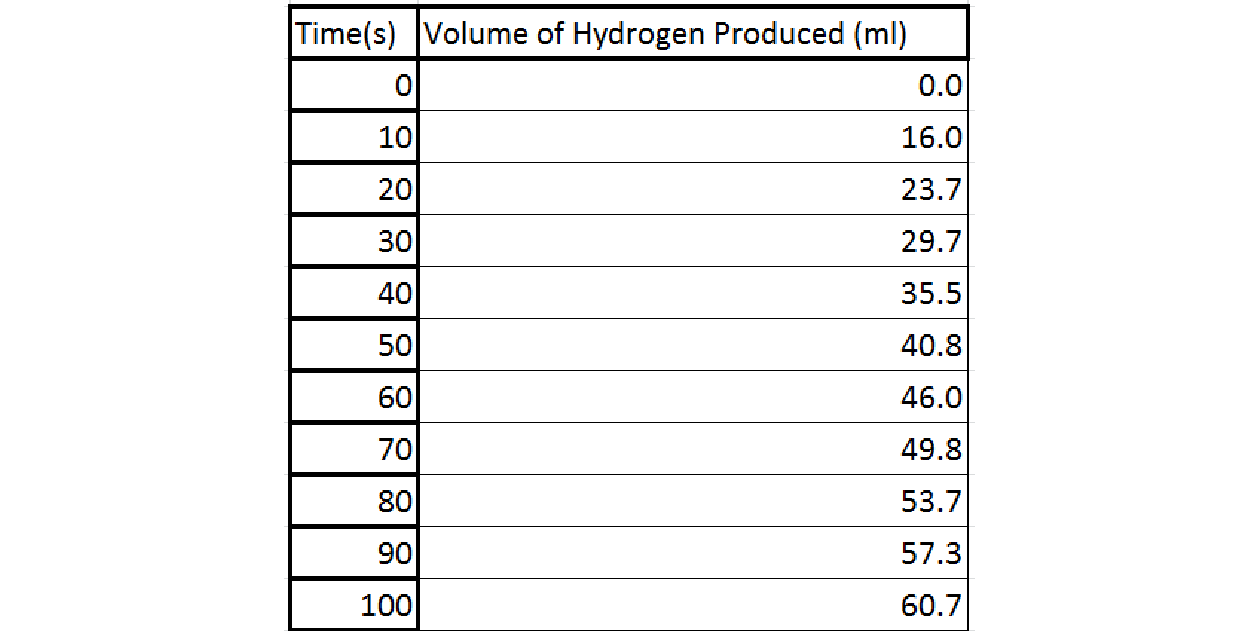
\includegraphics[width=\textwidth]{./Experiment/Images/4DifferentCatalysts/Copper.pdf}
    \caption{0.4 Molar Sulfuric Acid, 0.01 Molar Copper Sulfate and 1.0 g of Zinc} \label{fig:001MolarAverage}
\end{figure}

	\subsection{Nickel Sulfate}

\begin{figure}[H]
    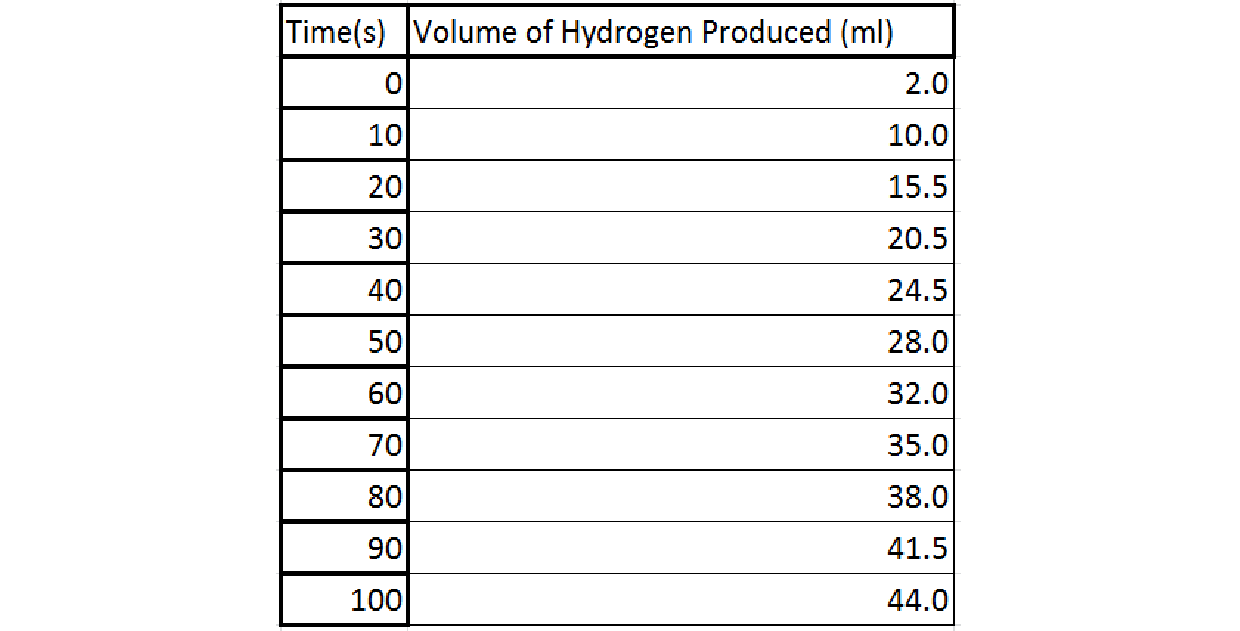
\includegraphics[width=\textwidth]{./Experiment/Images/4DifferentCatalysts/Nickel.pdf}
    \caption{0.4 Molar Sulfuric Acid, 0.01 Molar Nickel Sulfate and 1.0 g of Zinc} \label{fig:NickelRawData}
\end{figure}

	\subsection{Manganese Sulfate}

\begin{figure}[H]
    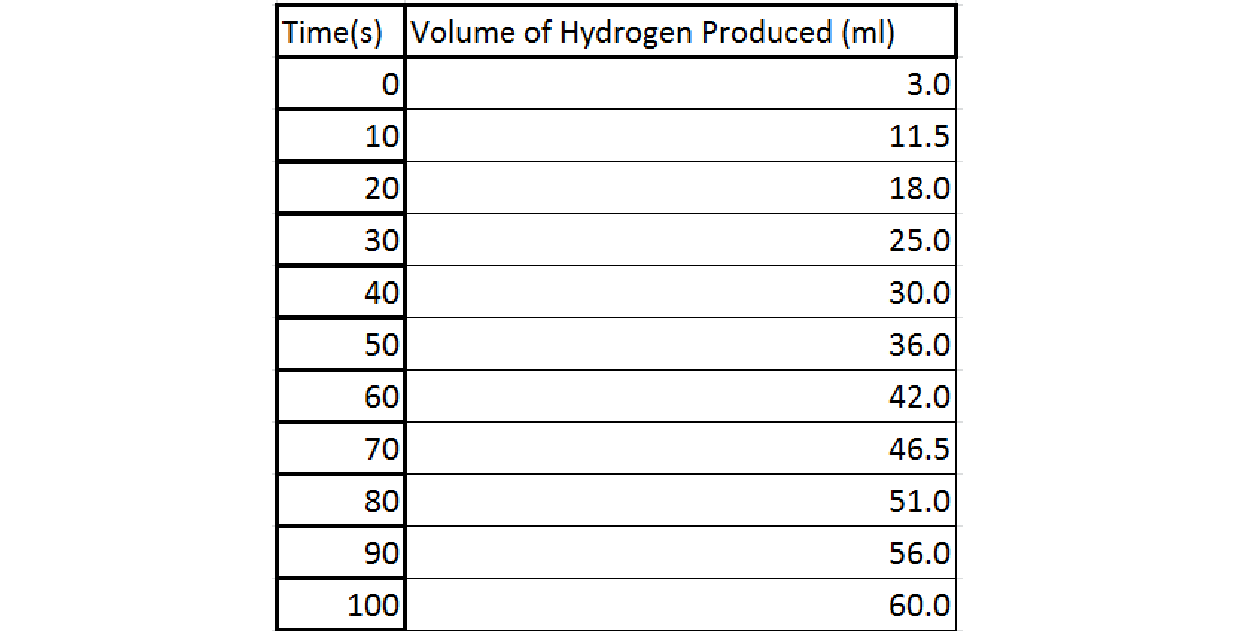
\includegraphics[width=\textwidth]{./Experiment/Images/4DifferentCatalysts/Manganese.pdf}
    \caption{0.4 Molar Sulfuric Acid, 0.01 Molar Manganese Sulfate and 1.0 g of Zinc} \label{fig:ManganeseRawData}
\end{figure}

	\subsection{Iron Sulfate}

\begin{figure}[H]
    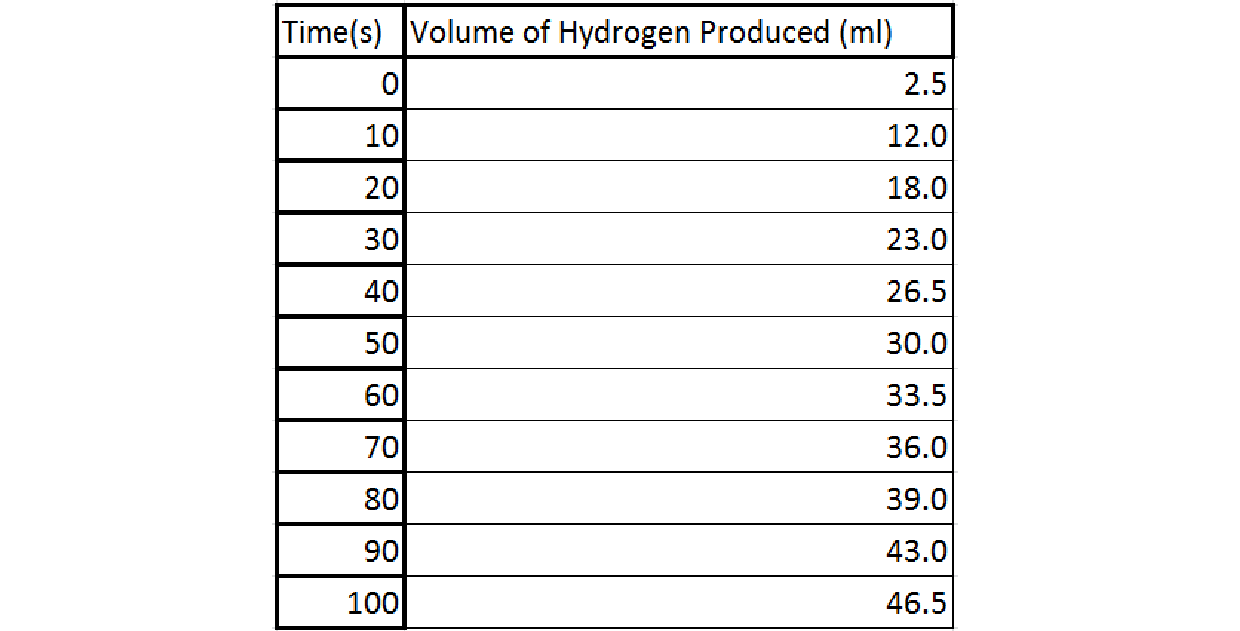
\includegraphics[width=\textwidth]{./Experiment/Images/4DifferentCatalysts/Iron.pdf}
    \caption{0.4 Molar Sulfuric Acid, 0.01 Molar Iron Sulfate and 1.0 g of Zinc} \label{fig:IronRawData}
\end{figure}


\section{Solubility of Hydrogen Experiment Series}

As shown by my non-catalyst experiment, it appears that the 3.2 molar experiment (Figure \ref{fig:32MolarSARawData} on page \pageref{fig:32MolarSARawData}) has a faster rate, and produces more hydrogen gas over 5 minutes, I began to wonder about the solubility of hydrogen within different acid concentrations. I predicted that the higher the concentration of acid, the higher the solubility of hydrogen. For this experiment I made sulfuric acid the excess reactant by using 0.1 g of zinc and 40 cm$^3$ of a range of different concentrations of sulfuric acid. The solutions used in this experiment were made up using the same method as I used for the rest of my solutions. This can be found in the 'Preparing Chemicals' section on page \pageref{Preparing Chemicals}.

	\subsection{1 Molar Sulfuric Acid}

\begin{figure}[H]
    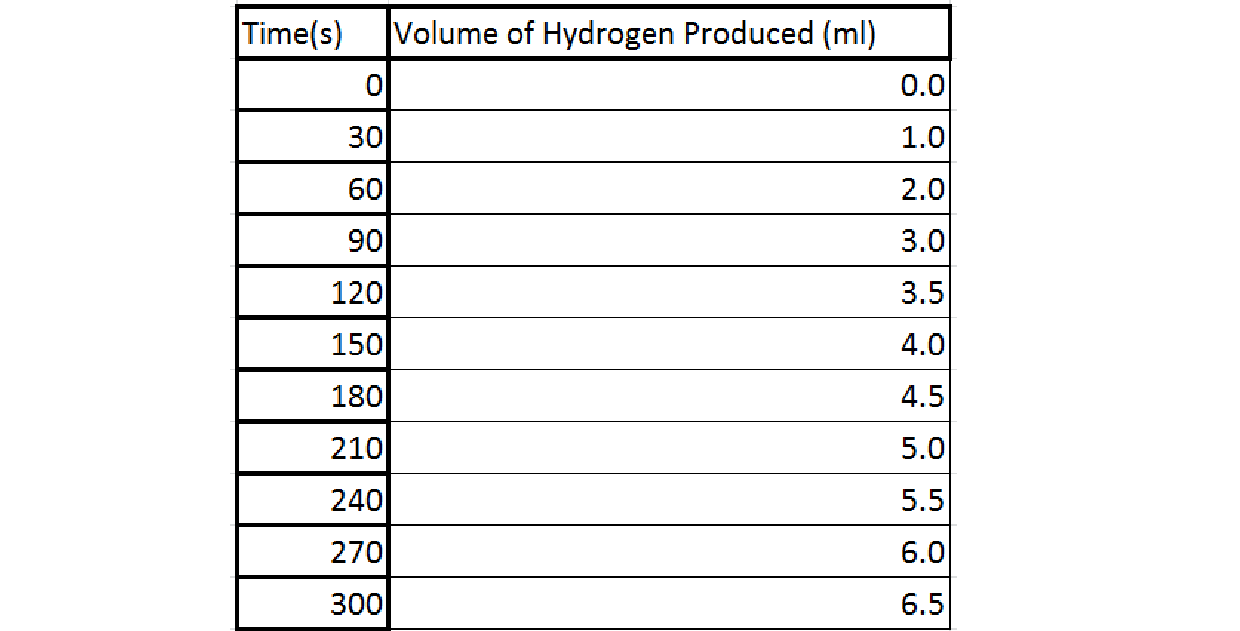
\includegraphics[width=\textwidth]{./Experiment/Images/5Solubility/1Molar.pdf}
    \caption{1.0 Molar Sulfuric Acid and 0.1 g of Zinc} \label{fig:1MolarSolubilityRawData}
\end{figure}

	\subsection{2 Molar Sulfuric Acid}

\begin{figure}[H]
    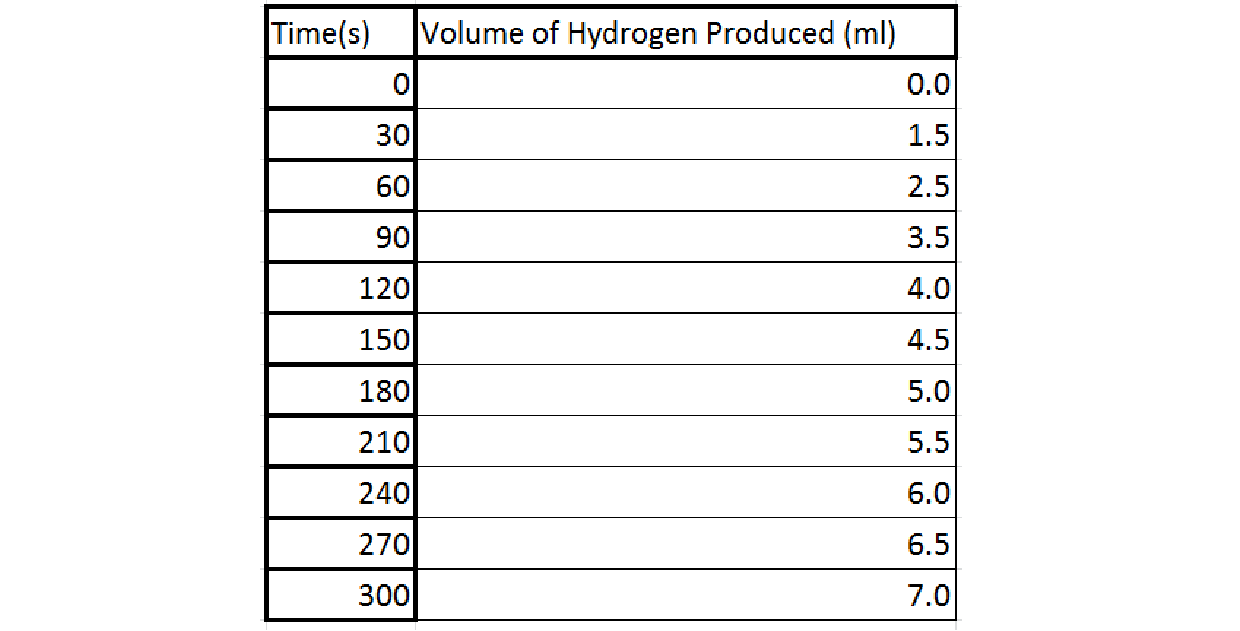
\includegraphics[width=\textwidth]{./Experiment/Images/5Solubility/2Molar.pdf}
    \caption{2.0 Molar Sulfuric Acid and 0.1 g of Zinc} \label{fig:2MolarSolubilityRawData}
\end{figure}

	\subsection{3 Molar Sulfuric Acid}

\begin{figure}[H]
    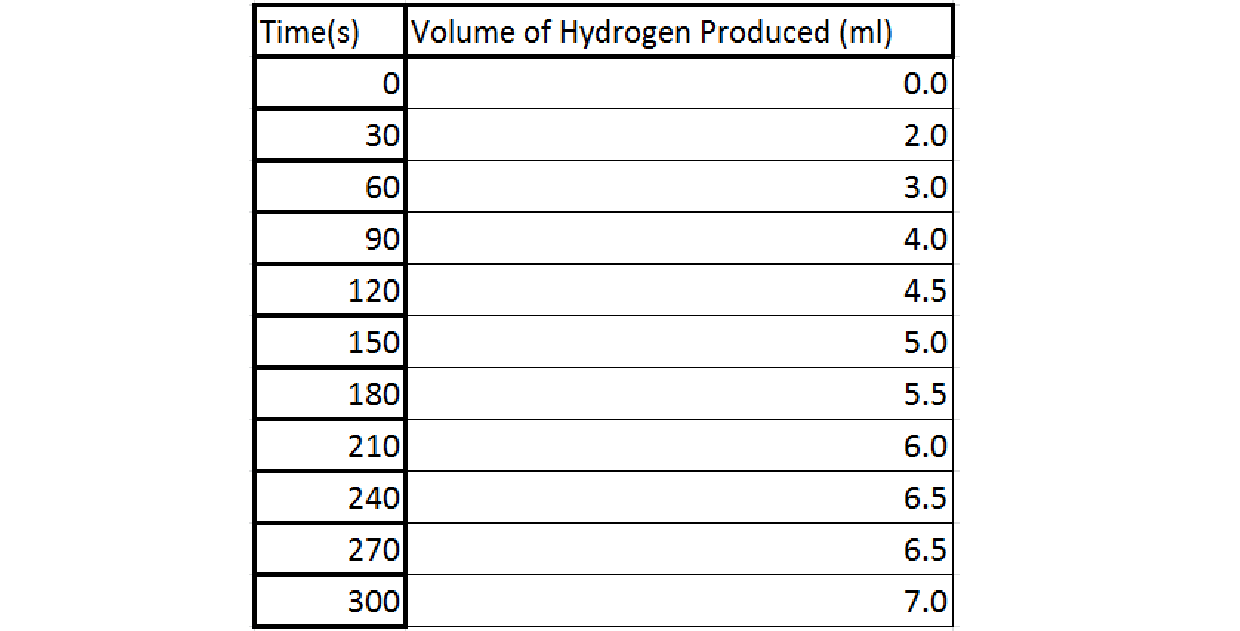
\includegraphics[width=\textwidth]{./Experiment/Images/5Solubility/3Molar.pdf}
    \caption{3.0 Molar Sulfuric Acid and 0.1 g of Zinc} \label{fig:3MolarSolubilityRawData}
\end{figure}

	\subsection{4 Molar Sulfuric Acid}

\begin{figure}[H]
    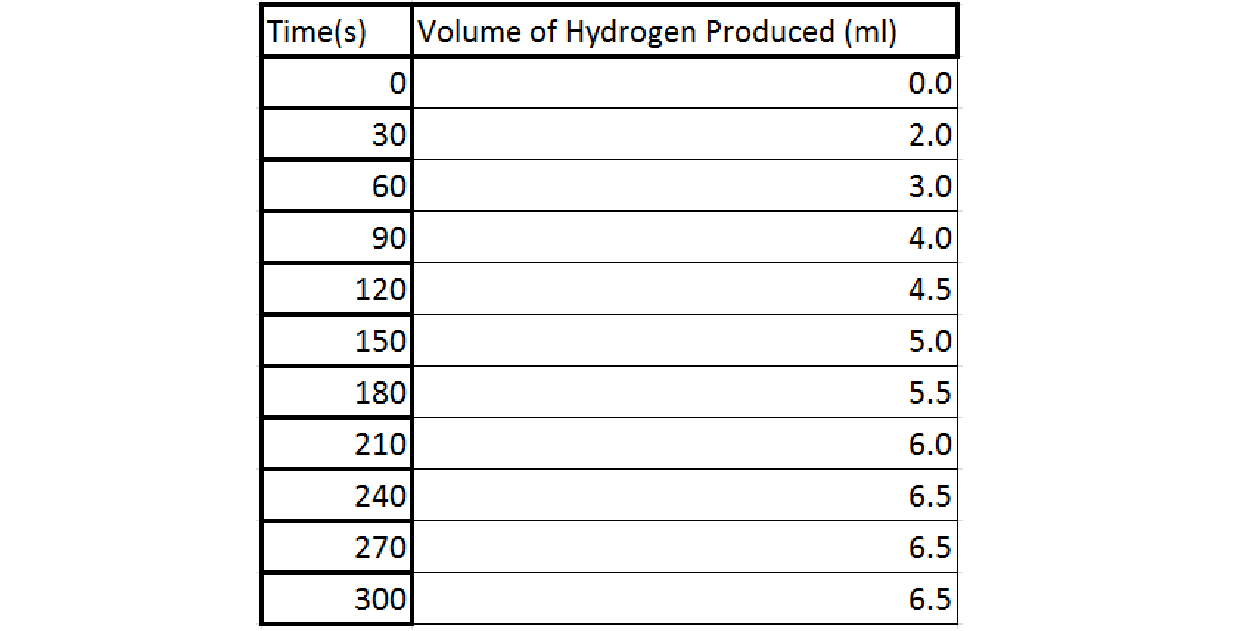
\includegraphics[width=\textwidth]{./Experiment/Images/5Solubility/4Molar.pdf}
    \caption{4.0 Molar Sulfuric Acid and 0.1 g of Zinc} \label{fig:4MolarSolubilityRawData}
\end{figure}